\documentclass[11pt]{article}
\usepackage{geometry}                
\geometry{letterpaper}                   

\usepackage{graphicx}
\usepackage{amssymb}
\usepackage{epstopdf}
\usepackage[square]{natbib}
\usepackage{amssymb, amsmath}
\usepackage{listings}
\usepackage[framed]{mcode}
\def \beq{\begin{equation}}
\def \eeq{\end{equation}}
\def \bea{\begin{eqnarray}}
\def \eea{\end{eqnarray}}
\def \bem{\begin{displaymath}}
\def \eem{\end{displaymath}}
\def \P{\Psi}
\def \Pd{|\Psi(\boldsymbol{r})|}
\def \Pds{|\Psi^{\ast}(\boldsymbol{r})|}
\def \Po{\overline{\Psi}}
\def \bs{\boldsymbol}
\def \bl{\bar{\boldsymbol{l}}}
\def \beq{\begin{equation}}
\def \eeq{\end{equation}}
\usepackage{float}

\DeclareGraphicsRule{.tif}{png}{.png}{`convert #1 `dirname #1`/`basename #1 .tif`.png}

%\title{Self-Organized Criticality}
%\author{Nishant Dogra, Michael Wild}
%\date{14.12.2012} 

\begin{document}




\thispagestyle{empty}

\begin{center}
\includegraphics[width=5cm]{ETHlogo.eps}

\bigskip


\bigskip


\bigskip


\LARGE{ 	Lecture with Computer Exercises:\\ }
\LARGE{ Modelling and Simulating Social Systems with MATLAB\\}

\bigskip

\bigskip

\small{Project Report}\\

\bigskip

\bigskip

\bigskip

\bigskip


\begin{tabular}{|c|}
\hline
\\
\textbf{\LARGE{Self-Organized Criticality and Phase Transitions }}\\
\textbf{\LARGE{in a Forest Fire Model}}\\
\\
\hline
\end{tabular}
\bigskip

\bigskip

\bigskip

\LARGE{Nishant Dogra, Michael Wild}



\bigskip

\bigskip

\bigskip

\bigskip

\bigskip

\bigskip

\bigskip

\bigskip

Zurich\\
December 2012\\

\end{center}



\newpage

%%%%%%%%%%%%%%%%%%%%%%%%%%%%%%%%%%%%%%%%%%%%%%%%%

\newpage
\section*{Agreement for free-download}
\bigskip


\bigskip


\large We hereby agree to make our source code for this project freely available for download from the web pages of the SOMS chair. Furthermore, we assure that all source code is written by ourselves and is not violating any copyright restrictions.

\begin{center}

\bigskip




\bigskip


\begin{tabular}{@{}p{3.3cm}@{}p{6cm}@{}@{}p{6cm}@{}}
\begin{minipage}{3cm}

\end{minipage}
&
\begin{minipage}{6cm}
\vspace{2mm} \large Nishant Dogra

 \vspace{\baselineskip}

\end{minipage}
&
\begin{minipage}{6cm}

\large Michael Wild

\end{minipage}
\end{tabular}


\end{center}
\newpage

%%%%%%%%%%%%%%%%%%%%%%%%%%%%%%%%%%%%%%%



% IMPORTANT
% you MUST include the ETH declaration of originality here; it is available for download on the course website or at http://www.ethz.ch/faculty/exams/plagiarism/index_EN; it can be printed as pdf and should be filled out in handwriting


%%%%%%%%%% Table of content %%%%%%%%%%%%%%%%%

\tableofcontents

\newpage

%%%%%%%%%%%%%%%%%%%%%%%%%%%%%%%%%%%%%%%



\section{Abstract}
In the scope of the ETH lecture "Modeling and Simulating Social Systems with Matlab", we attempt to produce a state of self-organized criticality in a forest-fire model. The concept is implemented as a cellular automata and several important data sets are extracted from the simulation. We describe the concept of self-organized criticality and cellular automata. We discuss the results found from the simulations and the implications of the input parameters on these. We try to explain what the quantitative characteristics of a SOC state in a forest fire model are and at which point such a state arises. 

\section{Individual contributions}
The Model with finite burning time was implemented by Nishant Dogra.
The Model with instantaneous burning time was implemented by Michael Wild.
The respective plots and results sections are also written in that way.
Both have contributed in writing the report and most of the sections are a work of collaboration and discussion.


\section{Introduction and Motivations}
\subsection{What is Self-Organized Criticality?}
Self-Organized Criticality involves 2 very important concepts: Self-Organization and Critical behavior\cite{ref3}. These 2 phenomenon arouse in various fields in very different forms.In certain class of systems, the dynamics can be very well explained by a few collective degrees of freedom. This dimensional reduction is termed as "Self Organization". It leads to evolution of global patterns in the system even though all the interactions are local. Let us take an example from the field of physics.Crystallization is the process of formation of crystals. It usually requires a small nucleus for the growth of the crystal. Once the nucleus is formed, crystal can grow on this nucleus. If we consider a particle which is going to crystallize on a given site, the choice of this site is decided only by the local environment seen by the particle. It does not depend on the particle on every other site on the crystal. But this local interaction leads to the formation of an ordered crystalline phase. Bird flocking is an example of self organization from the field of Biology.

On the other hand, there is another set of dynamical systems where the individual degree of freedom keep itself more or less in a stable balance and it is not possible to describe such a system by a few collective degrees of freedom. The key point in such systems is that the interdependence of various degrees of freedom make such systems very susceptible to noise. That's why, these systems can be called as "Critical". Critical state usually represent a point where 2 different phases occur simultaneously at the same time. A critical state has specific temporal and spatial signature. The power spectrum of the quantity representing the dynamics of the system is similar to that flicker noise. The spatial signature of a critical state is ``self-similarity'' which is what we find for the case of fractals.

Self-Organized criticality combines the above 2 concepts. In it, the dynamics of a physical system converge to a critical point independent of the bestowed boundary conditions. This critical point commonly is not the equilibrium point in a traditional, physical sense. We usually say that the \textit{critical point} is an attractor of the system dynamics. The concept is best understood by example, so we shall bring up a very educative one introduced first by \cite{ref3}. 
Imagine a sand pile in 2 dimensions. One can discretisze this pile into cells, which are denoted with the indices $n$. Each of those cells has an amount of sand grains on it, which is directly corresponding to the height $z_{n}$. Now we state the simple rule, that, if the difference in height between two neighboring cells becomes larger than a predefined limit, the higher cell will give grains to the lower cell (avalanche). Now every timestep, we drop a grain on cell one. Independent of the initial conditions, eventually, a straight slope will evolve. The critical point is reached if every difference between two neighboring cells is exactly the limit. What happens if we drop the next grain? Then the difference $z_{1}-z_{2}>p$ and one grain will drop on $z_{2}$. Subsequently, the difference $z_{2}-z_{3}$ will be too big and the process repeats until it hits the last cell. We therefore call a state critical if a yet so small disturbance can propagate throughout the whole system.
It is important to note here, that this critical state is \emph{not} the equilibrium state of the system, since that would be a flat surface. 

\subsection{Forest-Fire Model (FFM) as an example of Self-Organized Criticality}
As the name suggests, modeling of the ignition, propagation and extinction of fires in a forest is termed as Forest Fire Model (FFM). This model has been studied extensively as one of the dummy models to show Self-Organized Criticality. Historically, the first model for SOC was proposed by Per Bak,Kan Chen and Chao Tang \cite{ref4}. But it was later on shown that this model does not exhibit SOC state \cite{ref5,ref6}. Later, a slightly modified version of the original model was verified to exhibit SOC \cite{ref7}. After that, a lot of study has been performed on this model with various additive features. 

\subsection{Motivation to study Forest Fire Model}
Why is it important to study Forest Fire Model? Forest fire models apply to a wide range of problems and are therefore helpful in predicting the behavior of such systems. Self-Organized criticality is the concept that describes the dynamics of such models and the two fields are therefore closely connected. One has closely studied these effects to make better predictions about forest fires. The main problem was, that in most cases, even relatively small fires were extinguished by the authorities. Since that led to an \textit{overcritical state}, the probability for a huge, devastating fire rose quickly. This has happened in the past and had a serious impact on the ecosystem of those areas.
Since the problem of self-organized criticality has been understood, one has stopped to extinguish every little fire, therefore avoiding to reach an overcritical state at which the disturbance (a small fire) can propagate throughout the whole system (large-scale fire). 
The same ideas can be applied to a variety of problems such as disease spreading or urban planning.

\subsection{What do we want to know from the Forest Fore Model- The QUESTIONS}
First, we would like to understand what are the quantitative characteristics of a Self Organized Critical state in the Forest-Fire model? We would like to have a well defined idea regarding when does the Forest Fire model manifest SOC behavior and why. We would like to understand what are the various phases seen in a Forest Fire model besides the Self Organized Critical phase. It will be important to know what are the parameters characterizing the phase transition in the Forest Fire Model.
Some of the ambitious questions will be to understand the dependence of SOC of the Forest Fire model on the dimensionality of the Lattice or on the neighborhood selection on the grid.\\
It will also be interesting to find out if computational restrictions like finite size grids, periodic boundary conditions and cell updating procedures have a quantitative effect on the behavior of the model?



\section{Description of the Model}

\subsection{Cellular automata}

A cellular automata is a very powerful way of simulating problems which are defined by a set of rules. It is usually simulated on a grid, but not necessarily restricted to those geometrical constraints. The main characteristics are:
\begin{itemize}
\item Every grid point has a state

\item Grid points change their state depending on the neighbor states according to a set of rules

\item Random actions may be introduced
\end{itemize}

In the example of the FFM, each cell can have one of the following three states:
\begin{itemize}
  \item 0: A green tree
  \item 1: Empty site
  \item 2: Fire
\end{itemize}

The dynamics of the system is defined though the following rules.They are applied to every step as we go from 1 time step to the next.
\begin{enumerate}
\item If a tree is burning at a given time step (2), we make it an empty site during the next time step.
\item If a site is empty (1), a tree can be grown on it with a probability p. This means that if we found out a site to be empty, we generate a random number between 0 and 1. If the number is less than p, we change the state of the cell to 0, otherwise it stays an empty site.
\item If a site is a green tree (0), we burn this tree in the next step if:

\begin{itemize}
\item Either of its neighbors is a burning tree.
\item We generate a random number between 0 and 1, if it is less than f (lightening probability), we burn this tree.
\end{itemize}
\end{enumerate}

It is important to note that the Forest Fire Model does not only apply to forest fires as its name would suggest. A whole class of problems follows the same basic rules and can be treated accordingly. An example would be the spreading of a disease, where one can directly transform the above rules and states.

This model describes an SOC state in the regime where the ratio of p and f is very large and p itself is very small. An important question is how to characterize a state as an SOC state. This is described below.


The second approach to grid-based updating is with a second grid that stores temporary information. \cite{ref9}

\subsection{Understanding the SOC regime of Forest Fire Model}

For FFM to be an SOC, we need to ensure 2 things. One is that the probability of growing a tree should be much larger than the probability of lightening. We can intuitively think about the ratio of p and f as the number of trees growing between 2 lightening strokes.This condition ensures long range correlation in the system (which will lead to criticality) building out of purely local interactions (randomly growing trees). Another condition which we need to ensure is that the time needed to burn a large cluster should be much smaller than the time needed to grow a tree. This condition ensures invariance under a change of the length scale \cite{ref1,ref9}. The 2 conditions can be written together as:
\beq
T_{burn}(cluster_{max})<<p^{-1}<<f^{-1}
\eeq

\subsection{Critical Exponents}
Usually, a critical point is associated with certain power law distributions of various physical quantities characterizing a critical state. Power laws are functions of the form $ P(s) \varpropto s^{-\tau}$ . These functions are found in many data sets, such as the size distribution of cities in a certain area. Take any country, one will find one very large metropolis, a few large cities, many medium sized towns and a huge lot of small towns. Power laws have also prominently been found in data sets of earthquakes, where they apply almost perfectly, meaning that small earthquakes happen very often in respect to the frequency of big ones. Power laws imply that the frequency of a general data point is inversely proportional to its magnitude. 

At a critical point, the power laws are characterized by critical exponents which are the indicators of the critical state. They usually depend only on the dimension of the system and the nature of interactions/ dynamics involved. These exponents are independent of the initial condition and the size of the system. These critical exponents can be calculated either by mean field approaches or through numerical simulations. The mean field approach becomes more and more exact in higher and higher dimensions.

In context to the FFM, it is proposed as a way of quantifying the frequency of Fires with respect to their cluster size. 

\subsection{Key Parameters in FFM SOC}

To find out whether a basic FFM exhibits SOC behavior, we need to define a set of parameters which serves as indicators for the desired analysis. 
\begin{itemize}

\item The time needed to burn down a forest cluster: This is heavily dependent on the form of the implementation. We can implement it in a way where we will have an instantaneous fire which essentially takes no time to burn and just resets all the connected trees. If however, we choose the form of a visible fire, meaning that the ratio $f/p\ll1$  is not 0  in limit and that it takes the fire one time step to advance a grid cell, then the time needed to burn a forest cluster is an important variable we need to extract from the simulation.


\item Number distribution of the size of clusters: Here we first need to define what a cluster is. A cluster is a set of neighboring cells (Von Neumann neighborhood) all obtaining the same state. When we talk about forest clusters, we of course mean connected trees. In the implementation where the fire spreads infinitely fast, the forest cluster containing the igniter cell is the same as the burnt area. The size distribution therefore is a very good indicator for the fire size distribution. 

\item The mean number of forest clusters in a unit volume $n(s)$ , where s  is the number of trees in a cluster. 

\item The radius of a cluster, it is defined as the root mean squared distance of all the elements of a cluster from the mean. It gives an estimate of the size of cluster. 

\item Number of fires per unit time step: This is a tuning parameter of the model.

\item Correlation length.
\end{itemize}
We have tried to implement the model in a way that the measurement of these desired variables is possible with the least needed effort.


\section{Implementation}
As discussed before, there are two main implementation methods for the model: One way is to update the whole grid every time step, whereas the second method picks a cell randomly at every time step an only updates the chosen one. One of us worked on the first method and the other one worked on the second method.

\subsection{Grid Based Updating}
The algorithm for grid initialization looks like:
\begin{verbatim}
Grid(N,N)=zeros(N,N)
rand_grid=rand(N,N) // we generate a grid of random numbers
m=1;
while m<=size(Grid,1) // Loop over all y-coordinates
		n=1;
		while n<=size(Grid,2) // Loop over all x-coordinates
			if rand_grid(m,n)<k //If the random number for a site is less than k, 
													//we make the site empty, else it has a tree
				Grid(j,k)=1   		// chossing different k will lead to different 
													//initial state of the grid
			end
		end
end
\end{verbatim}
Basically, we initialize the grid with trees and empty sites distributed randomly on the grid.
The updating of the grid based on the simple rules described above can be done in 2 different ways. One is when we make a copy of the current grid ($Grid\_copy$) and then update the current grid using this $grid\_copy$. The other is that we use the current grid (which is being updated) as the one which also responsible for updating. The 2nd procedure require us to pick the sites randomly and update them, but it will be hard to keep track about the sites which have been updated at a time step. In our simulations, we follow the first procedure whose algorithm is described below: 

\begin{verbatim}
it=1:
while it<=Iter // Loop over all time steps
    Forest_grid_temp=Forest_grid;  //Forest_grid_temp is the copy
    //which is used to update the grid at the next time step.
		// we need to take care that the neighbors of every cell are correct 
		//as based on the periodic boundary condition. 

		//This has been handled by making the size of the copy as 2 units 
		//larger in each of the dimensions    
		
    Copy the first column of Forest_grid to last column of Forest_grid_copy
    Copy the last column of Forest_grid to first column of Forest_grid_copy
    Copy the first row of Forest_grid to last row of Forest_grid_copy
    Copy the last row of Forest_grid to first row of Forest_grid_copy
    m=2;  //looping over the Forest_grid and its copy, 
    while m<N
        n=2;
        while n<N
            if Forest_grid_temp(m,n)==2
                Forest_grid(m,n)=1;
              //a fire becomes an empty site  
              
            elseif Forest_grid_temp(m,n)==1
                emp=emp+1;
                if rand(1,1)<p
                    Forest_grid(m,n)=0;
                end
              //an empty site becomes a tree if a generated random no. is <p
            else
                if (rand(1,1)<f || Forest_grid_temp(m-1,n)==2 || 
                Forest_grid_temp(m+1,n)==2 || Forest_grid_temp(m,n-1)==2 ||
                 Forest_grid_temp(m,n+1)==2)
                					    Forest_grid(m,n)=2;
                //if any of the neighbours of the current site is burning or a
                //random number is generated which is greater than lightening 
                //probability, we burn the tree.
                end
            end
            n=n+1;
        end
        m=m+1;
    end
    it=it+1
end
\end{verbatim}
One of the important reasons why we made another model is that the algorithm is quite slow because of all the loops and if-statements,we are using.

The next important thing which we need to find out is indexing uniquely all the clusters of trees. The algorithm is described below:
\begin{verbatim}
Index=3;
m=1;  //looping over the Forest_grid and its copy, 
while m<N
   n=1;
   while n<N
   		if Forest_grid(m,n) is an un-indexed tree
   				we search all its neighbors to find the smallest index
   						if index is found,
   									Forest_grid(m,n)=index;
   									We also update the index of all the nearest
   									trees with this index
   						if index is not found,
   									Forest_grid(m,n)=Index;
   									We also update the index of all the nearest
   									trees with this Index
   									Index=Index+1;
   						end						
			end
	end
end
//The above loop will be sufficient if we have absorbing boundary conditions.
//Periodic boundary condition requires that we should check all the indexing
//again
m=1;  //looping over the Forest_grid and its copy, 
while m<N
   n=1;
   while n<N
   		if Forest_grid(m,n) is a tree
   				we search all its neighbors to find the smallest index
   				If the index of any of the neighbors or the Forest_grid(m,n)
   				is different than this smallest index, we replace all the trees
   				of that index with this smallest index				
			end
	end
end

for i=1:t // Loop over all timesteps
    for j=1:size(Grid,1) // Loop over all y-coordinates
        for k=1:size(Grid,2) // Loop over all x-coordinates
            if Grid(j,k)==0 //If the grid point is empty
                //Grid(j,k)=1 with some probability p
            end
        end
    end
    for j=1:size(Grid,1) // Loop over all y-coordinates
        for k=1:size(Grid,2) // Loop over all x-coordinates
            //if Neighbor(j,k)==3 // If grid neighbor is burning
                Grid(j,k)=2 // Set current grid point on fire
            end
        end
    end
    for j=1:size(Grid,1) // Loop over all y-coordinates
        for k=1:size(Grid,2) // Loop over all x-coordinates
            if Grid(j,k)==3 // If Grid point is burning
                Grid(j,k)=0; // Turn it into an empty site
            end
            if Grid(j,k)==2 // If grid point is ignited
                Grid(j,k)=3; // Turn it into an empty site.
            end
        end
    end
end
\end{verbatim}

Several things are to note here:
\begin{itemize}
\item Commands with // or  in front are not implemented exactly like that. Check the appendix for the complete source code.
\item We need several spatial loops in order to successfully suppress updating fragments like infinite fire propagation speed in updating direction. 
\item For the same reason, we need a differention between newly ignited (state 2) and burning (state 3) trees. 
\item The Algorithm is quite slow because of all the loops and if-statements.
\end{itemize}

Once the indexing is done, we can simply count the number of trees corresponding to a given index and can find out the number of number of clusters of a given size (where by size, we mean the number of trees in the cluster).

Calculation of the radius of a cluster is little subtle. Naively, it just the root-mean squared distance of all the elements from the cluster mean. The formula can be simplified as:
\beq
R=\sqrt{\frac{1}{N}\sum{x_{i}^{2}}-\frac{1}{N}(\sum{x_{i}})^2}
\eeq  
This would have worked well if we have absorbing boundary conditions, but since our boundary is periodic; there can be possible a cluster which is going over the boundary. In that case, above formula can lead to a cluster mean which is outside the cluster. In such a situation, we need to rotate our grid to calculate the cluster radius properly and efficiently. The underlying idea is very simple. If you are scanning through different columns (rows) from left to right (top to bottom), you should get an element of a cluster in every column since the starting column for that cluster. In case, there is a break, it implies that you have cluster going though the edges, otherwise it cant be a cluster. Another important property of a cluster going through their boundary is that it should have a member in the leftmost (topmost) and rightmost (down most) column (row). We exploit these in the following algorithm:\\

\begin{verbatim}
//Column shift
define variables F and ml for every cluster index
initialize F and ml with zero for every cluster
m=1
while m<=N  %going through all the columns
	n=1;
	while n<=N  //going through all the rows of a given column
			if the current element is a tree,store the index of current 
			element in variable cl
			if F(cl)==0
					//this is the first column where an element of this cluster appears.
					if m~=1
							F(cl)=3;
							//this implies that this cluster cannot be connected via the boundary
					else
							F(cl)=1;
							ml(cl)=m;
				  end
			elseif F(cl)==1
					if m~=ml(cl)+1
						//this is the case when we have atleast one column in between where no
						//element of the given cluster is found and this can happen only if
						//the cluster passes through the boundary.
							  F(cl)=2;
					end		  
					ml(cl)=m;
			end
	end
end			
//The column shift needed for a given cluster can be calculated as:
if F(cl)==2
			shift_col(cl)=N+1-ml(cl)
else
			no shift
end									  

//An exactly similar procedure is followed to calculate the row shift for every cluster 
//index where we go though all the columns for a gicen row and very all the rows.

\end{verbatim}

\subsection{Random Based Updating}
In a random based updating implementation, at the beginning of every time step, one random cell is chosen. It then checks for the rules of the model and acts accordingly. In order to see fires, we need to have instantaneous burning, which is actually permitted by the model. However, it changes the dynamics of the system drastically. But more about that later. The following steps are taken for each timestep:

\begin{enumerate}
\item Choose a single cell
\item If cell is empty, grow a tree with probability $p$
\item If cell is a tree, with probabiltiy $f$, burn it and the connected cluster
\end{enumerate}
In Matlab, this looks something like this:

\begin{verbatim}
for i=1:t // Loop over all timesteps
(j,k)=ceil(Grid_Size*rand(1,2)); // Choose a random cell
	if  Grid(j,k)==0 % If the cell is empty
		//With some probability p set G(j,k)==1;
	end
	if Grid(j,k)==1 // If the cell is alive
		//with some probability f execute burn(j,k);
	end
end
\end{verbatim}

This implementation of the forest fire model has several advantages:
\begin{itemize}
\item There are no problems due to updating processes
\item Much shorter implementation
\item Easier to extract data
\end{itemize}
The last point is to be explained more extensively: Every time a tree ignites, the whole connected cluster is burned down. Since the whole process happens in a single timestep, there are no big issues.
This implementation, however, also comes with quite a big disadvantage: It fails to capture dynamics. This leads to a quasi-static simulation. We are not totally sure how this affects the simulation results.

\subsubsection{keeping track of the clusters}
Keeping track of the different clusters was more difficult than we thought at first, but we managed to find an elegant solution. It works by keeping a second grid which stores all the cluster indices. This has several advantages:
\begin{itemize}
\item if a new tree grows, we can just look at the neighbor cluster index to determine the current cell index
\item if a tree burns, we simply delete all the trees with the same index as the burned tree.
\end {itemize}
 \paragraph * {Problems and Solutions}
Problems arose quickly. Here is a short summary of all the major problems and the corresponding solutions:
\subparagraph {Storing the indices}
The problem here was to find a way to store all possible cluster indices and their availability. Since the maximum number of clusters can be easily found to be $Nc_{max}= \frac{G^2}{2}$  (imagine a perfect chessboard-layout filling half of the grid; if one more is added, they combine into a bigger cluster), we already knew the size of the vector. The final format was a Matrix with $Nc_{max}$ Columns and 2 rows. The first row would simply store all the possible indices from 1 to $Nc_{max}$ and the second row would store the corresponding binary information about the availability.
\subparagraph{growing a tree between two clusters}
It is simple to determine the cluster index of a new tree if there is just one neighbor. The big problem arises if there are more than two neighbors with \emph{different} cluster indices. The solution to this problem was that we set the index as the lower of both neighbors and changed the whole cluster with the higher index to the lower one. This was relatively easy to do by using the matlab built-in function |ismember| which searches for all entries with a certain value and returns a matrix containing only that information. 

\subsection{The \emph{neighbor} function}
The \emph{neighbor} function is the same for both implementations. It takes the current cell coordinates  $(j,k)$ and returns a vector containing the coordinates of its direct neighbors. It works like this:
\begin{verbatim}
Set all neighbors to standard
// Ex: West_X=j-1; West_Y=k;
Treat Special cases
// Ex: if j==1
// West_X=size(Grid,1);
\end{verbatim}
Note that the \emph{neighbor} function creates periodic boundary conditions. 

\subsection{Saving the data}
Because we were doing a lot of parameter sweeps and thus generating a lot of data, it was crucial to implement an automatic data saving procedure. This would store all the relevant information of a single simultation in a custom matlab struct and save the important figures. We also created a custom naming concept which allows for quick search for the desired data. All simulation results are named after their input parameters: 


\section{Simulation Results and Discussion}
\subsection{Traditional Forest Fire Model}

In this section, we will explain our results and understanding of the traditional model of Forest fire. Here we can consider 4 different regimes. 
\begin{itemize}
\item small p ($< 0.001$) and small $\frac{p}{f}$ ($\approx 1$)
\item large p ($< 0.001$) and large $\frac{p}{f}$ ($\approx 10^4$)
\item large p ($< 0.001$) and small $\frac{p}{f}$ ($\approx 1$)
\item small p ($< 0.001$) and large $\frac{p}{f}$ ($\approx 10^4$)
\end{itemize}

Let us first try to understand what we expect intuitively for these cases. In the first case, we will have growth rate of trees to be very small and comparable rate of fires.(The smaller values of usually make the time scale of variation of the system very large.) As a result, we don't expect long-range correlations for the system to build up.\\

\begin{figure}[H]
\centering
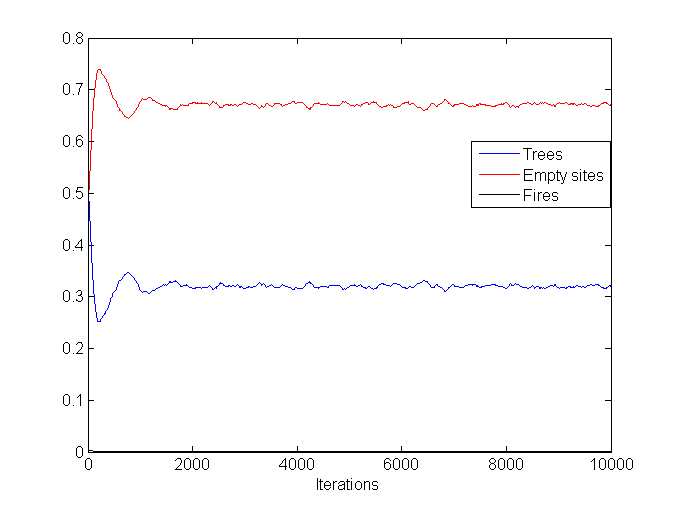
\includegraphics[width=0.9\textwidth,keepaspectratio=true,]{Pictures/case1_size_500.png}
\caption{$N=500$, $\ p=0.001$, $\frac{p}{f}=10$(Case1)}
\end{figure}

In the second case, system will try to build long correlations since the tree growth rate is large. But since p is large, it won't be possible to make the system critical because before a large cluster is burnt by the fire, trees will start growing again in the cluster and the system won't really be in a critical condition.\\

\begin{figure}[H]
\centering
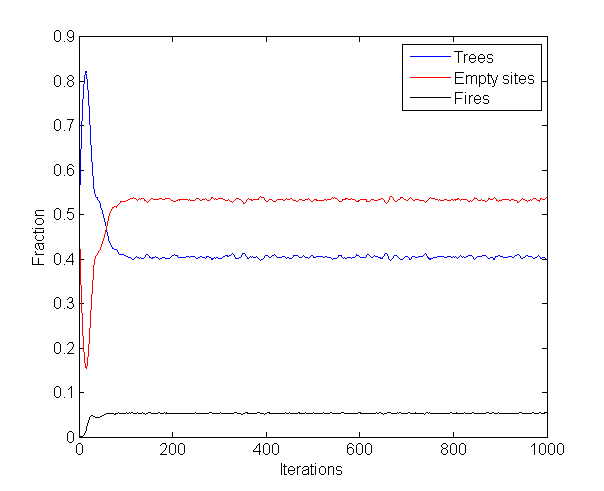
\includegraphics[width=0.9\textwidth,keepaspectratio=true,]{Pictures/case2_size500_1000iter_p_0point1_ratio_1000.png}
\caption{$N=500$, $\ p=0.1$, $\frac{p}{f}=1000$(Case2)}
\end{figure}

The 3rd case takes the worst part of the above 2 cases. The large tree growth rate don't let the system to become critical. The small $\frac{p}{f}$ wont let the formation of long range correlation in the system and avoid from making the system being critical.\\
\begin{figure}[H]
\centering
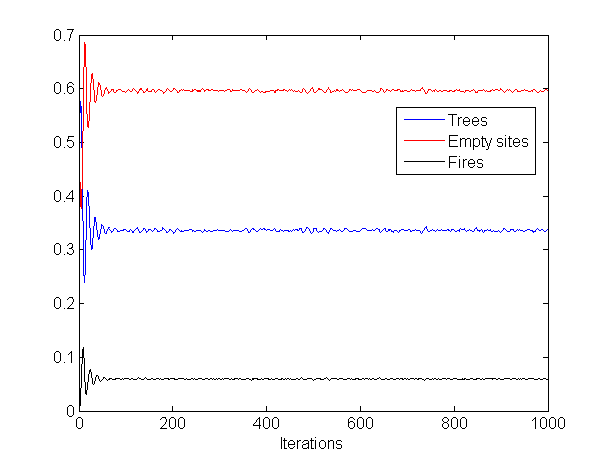
\includegraphics[width=0.9\textwidth,keepaspectratio=true,]{Pictures/case3_size500_1000iter_p_0point1_ratio_10.png}
\caption{$N=500$, $\ p=0.1$, $\frac{p}{f}=10$(Case3)}
\end{figure}

In conclusion, these 3 cases are some sort of equilibrium populations where system never becomes critical.

The final case is the one we are interested in. Since $\frac{p}{f}$ is large, large correlations can be built in the system. Since p is small, formation of large correlations make the system critical.
\begin{figure}[H]
\centering
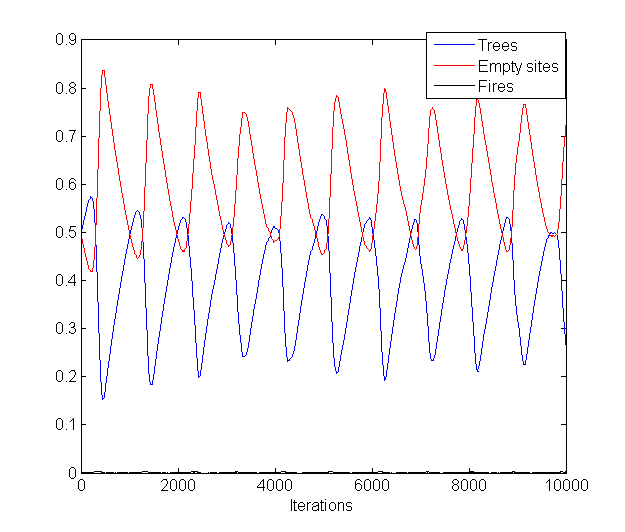
\includegraphics[width=0.9\textwidth,keepaspectratio=true,]{Pictures/case4_size500_10000iter_p_0point001_ratio_1000.png}
\caption{$N=500$, $\ p=0.001$, $\frac{p}{f}=1000$(Case4)}
\end{figure}

From the way we model our system (we are considering case 4 above), it is very difficult to find out whether for a given set of parameters the time required to burn the biggest cluster in system is much smaller than the time needed to grow a tree. But there is a very simple qualitative way to see this through the variation of various fractions as the system evolves. When an event of lightening happens in the system, the fraction of empty sites grows quickly. But shortly after that when the cluster is fully burnt, the trees again start growing and the fraction of empty sites start to decrease again. If the slope of the slope of increase of the fraction of empty sites when the fire is burning the cluster is much larger than the slope of decrease of fraction of empty sites when the trees start growing, it implies that the cluster burning process is almost instantaneous in comparison to the tree growth. Hence, in the 4th case we expect the system to be in SOC state. In the following figure, we show the case when the system is critical in the sense that long range correlations are forming (a fire is burning big cluster) but the fire is not instantaneous in comparison to the tree growth rate.

\begin{figure}[H]
\centering
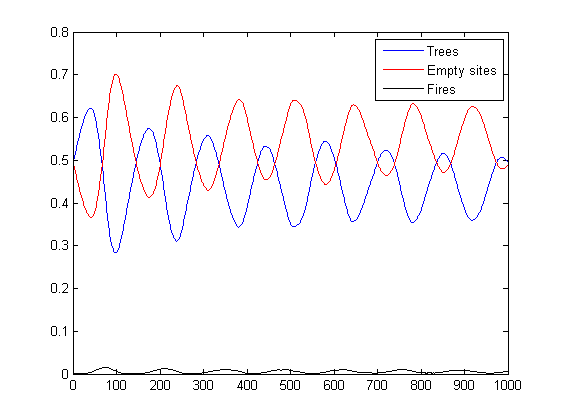
\includegraphics[width=0.9\textwidth,keepaspectratio=true,]{Pictures/case4_size500_10000iter_p_0point01_ratio_1000.png}
\caption{$N=500$, $\ p=0.01$, $\frac{p}{f}=1000$(Case4)}
\end{figure}



An important point to make here is how the size of the grid affects this self-organized critical state. We see that if the grid is big, we will be having larger long range correlations. It will take larger time for a fire to burn a cluster and hence the regime where the cluster burning is almost instantaneous as compared to tree growth will require lower values of p.
This has been shown in the following figure by considering a much smaller grid size as for the case 4 but same parameters.
\begin{figure}[H]
\centering
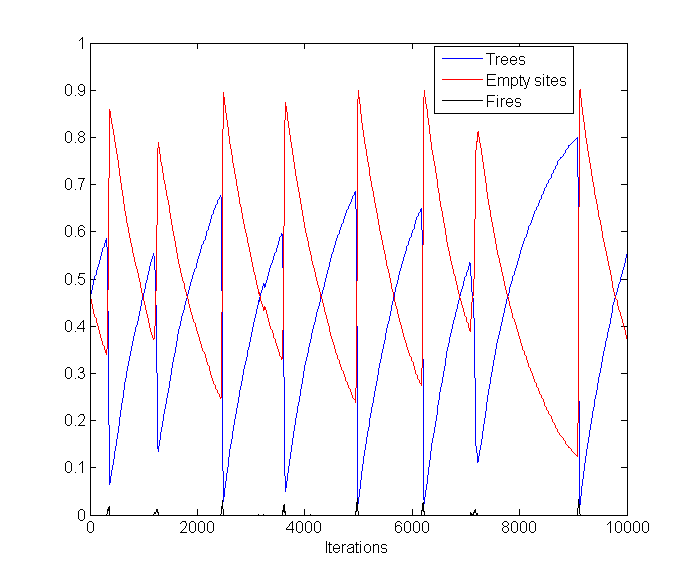
\includegraphics[width=0.9\textwidth,keepaspectratio=true,]{Pictures/case4_size50_10000iter_p_0point001_ratio_1000.png}
\caption{$N=50$, $\ p=0.001$, $\frac{p}{f}=1000$(Case4)}
\end{figure}

Now, we plot the radius distribution and the frequency of clusters as a function of number of trees in the cluster. Thes eare plotted in the figures below.


\begin{figure}[H]
\centering
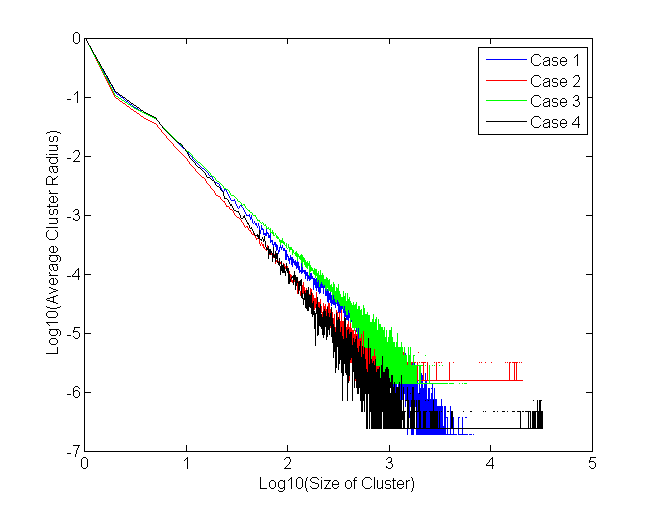
\includegraphics[width=0.9\textwidth,keepaspectratio=true,]{Pictures/frequency_distribution_4_different_cases.png}
\caption{$N=200$, Frequency Distribution}
\end{figure}

\begin{figure}[H]
\centering
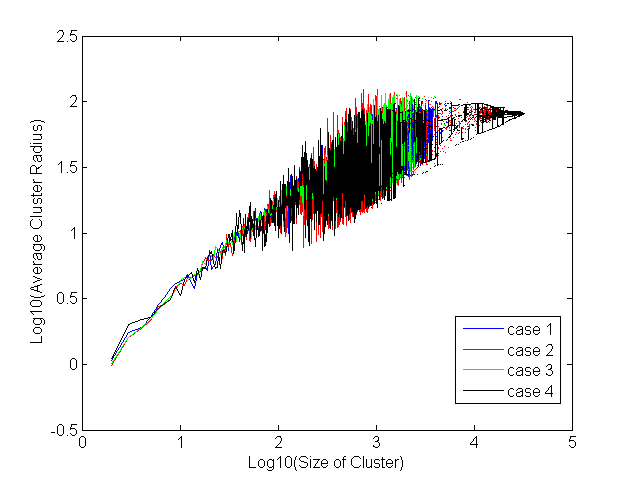
\includegraphics[width=0.9\textwidth,keepaspectratio=true,]{Pictures/radius_4_cases.png}
\caption{$N=200$, Radius Distribution}
\end{figure}

Here we see one of the important drawbacks of this model. Since the algorithms are a bit slow, within our computational limits we cant distinguish the 4 cases from these distributions. This is the reason why we worked on another implementation of the forest fire model which is much faster than this traditional implementation.

\subsection{The Second Implementation}
\subsubsection{Cluster Radius}
The Cluster Radius is defined as the root mean of all the distances of all cells of a cluster to their common center. According to the literature, the cluster radius distribution should exhibit a power law behavior and therefore form a straight line in a log-log-plot. We were having some small issues with the cluster radius calculation, but ended up with something that very much resembled such a straight line, as can be seen in Fig.\ref{raddist1}. The "transient" behavior at large cluster radii is mostly due to too small simulation duration. We did longer simulations, but that constrained the grid size since at some point, the available memory would be gone. 
\begin{figure}[H]
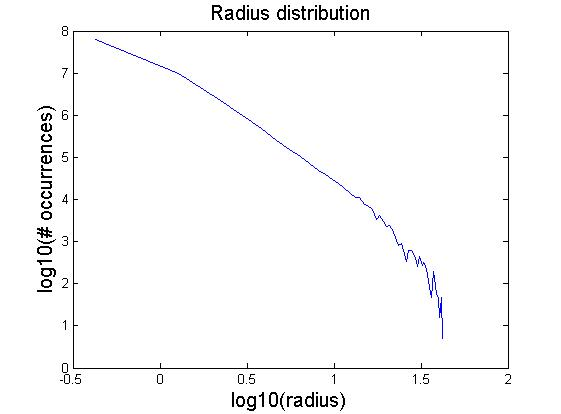
\includegraphics[width=0.9\textwidth,keepaspectratio=true]{Pictures/RadiusDist_100_200_1M.jpg}
\caption{Cluster radius distribution ($N=100$, $\Theta=200$, Sim Time 1'000'000)}
\label{raddist1}
\end{figure}
What we could find was a best slope estimation, which turned out to be around $\beta \approx -3$ for the parameters seen in Fig.\ref{raddist1}. Since the cluster radius distribution seems to be the most important attribute of the simulation, we thested the effects of various parameters on the simulation by the respective resulting cluster radius distributions. This will be discussed later.


\subsubsection{Cluster Size}
The cluster size is another variable that we can easily measure. Here is a log-log-histogram of a simulation:
\begin{figure}[H]
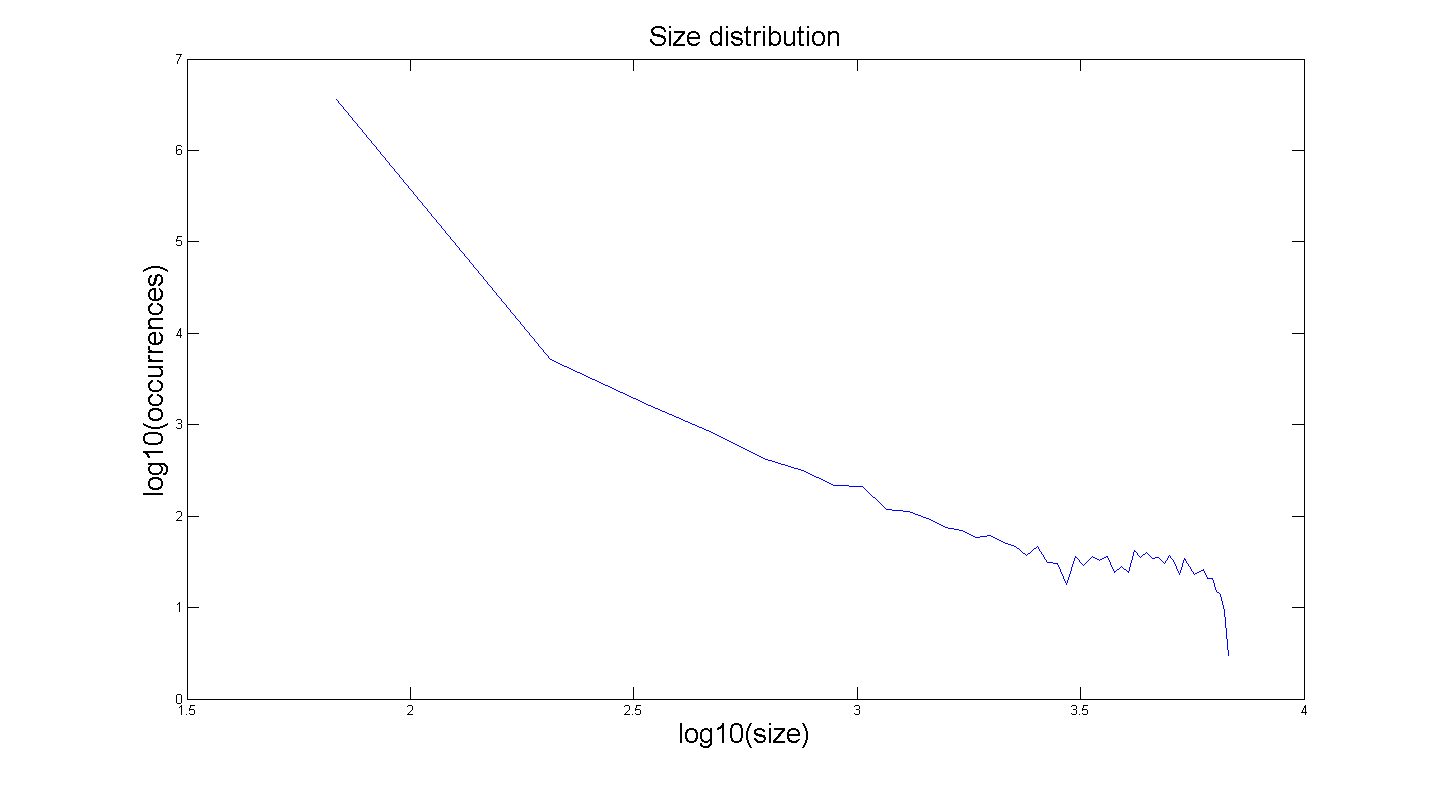
\includegraphics[width=0.9\textwidth,keepaspectratio=true]{Pictures/Size_dist_1.png}
\caption{Cluster size distribution ($N=100$, $\Theta= 1000 $, Sim Time 500'000  ) }
\end{figure}

%\subsubsection{Effect of different parameters}
\subsubsection{Effect of p and f}
In the case where the time needed to burn down a cluster is significantly shorter than the time required to grow one, these effects happen on a separated timescale. Looking at fire incidents on a "growth"-timescale, fires spread instantaneously. The question was, would the values of p and f have any effect on the simulation outcome if the ratio $f/p$ is kept constant? 
We tried to explain it intuitively: the larger the value of p is, the smaller the "time resolution". If it takes $n$ timesteps to grow a certain cluster at $p=1$, intuition says it will take $2n$ timesteps at $p=0.5$. Given that the lightning factor f varies proportionally, it also takes twice the time for a fire to happen. Of course, we are talking about expected values here, but since the whole process is a stochastic one by nature, it all pans out in the end. We ran a bulk simulation to verify this claim and ended up with the results seen in Fig.\ref{varpctheta}.
\begin{figure}[H]
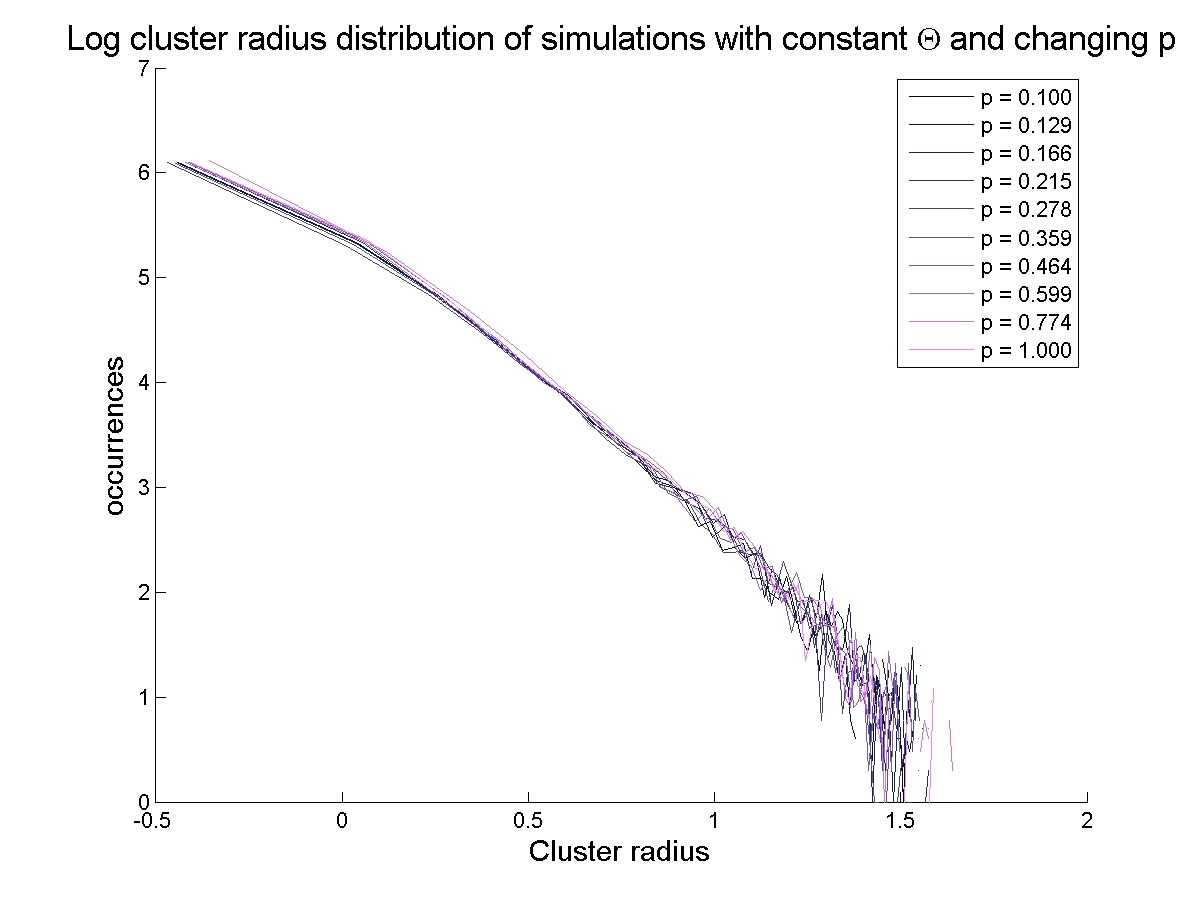
\includegraphics[width= 0.9\textwidth,keepaspectratio=true]{Pictures/varpconsttheta.jpg}
\caption{Log cluster radius distributions of simulations with constant $\Theta$ and changing p}
\label{varpctheta}
\end{figure}
The results came out as expected. Note that we are only interested in the \emph{slope} of the curves, not the position of the curves themselves. In fact, the simulations in Fig.\ref{varpctheta} were all run for a different number of timesteps to adjust for the "time resolution", so that they fit nicely on top of each other and the resemblance is visible. We therefore conclude that at constant values of $\Theta$, the values of p and f are not significant as long as they dont get too small. But in the case of instantaneous fire propagation, $p=1$ is the obvious choice to maximize simulation speed.

\subsubsection{Effect of $\Theta$}
Since an SOC state is also characterized in a way that $\Theta$ should be the only relevant tuning parameter, we ran some bulk simulations to test this statement. The results can be seen in Fig.\ref{varthetaconstp}.
\begin{figure}[H]
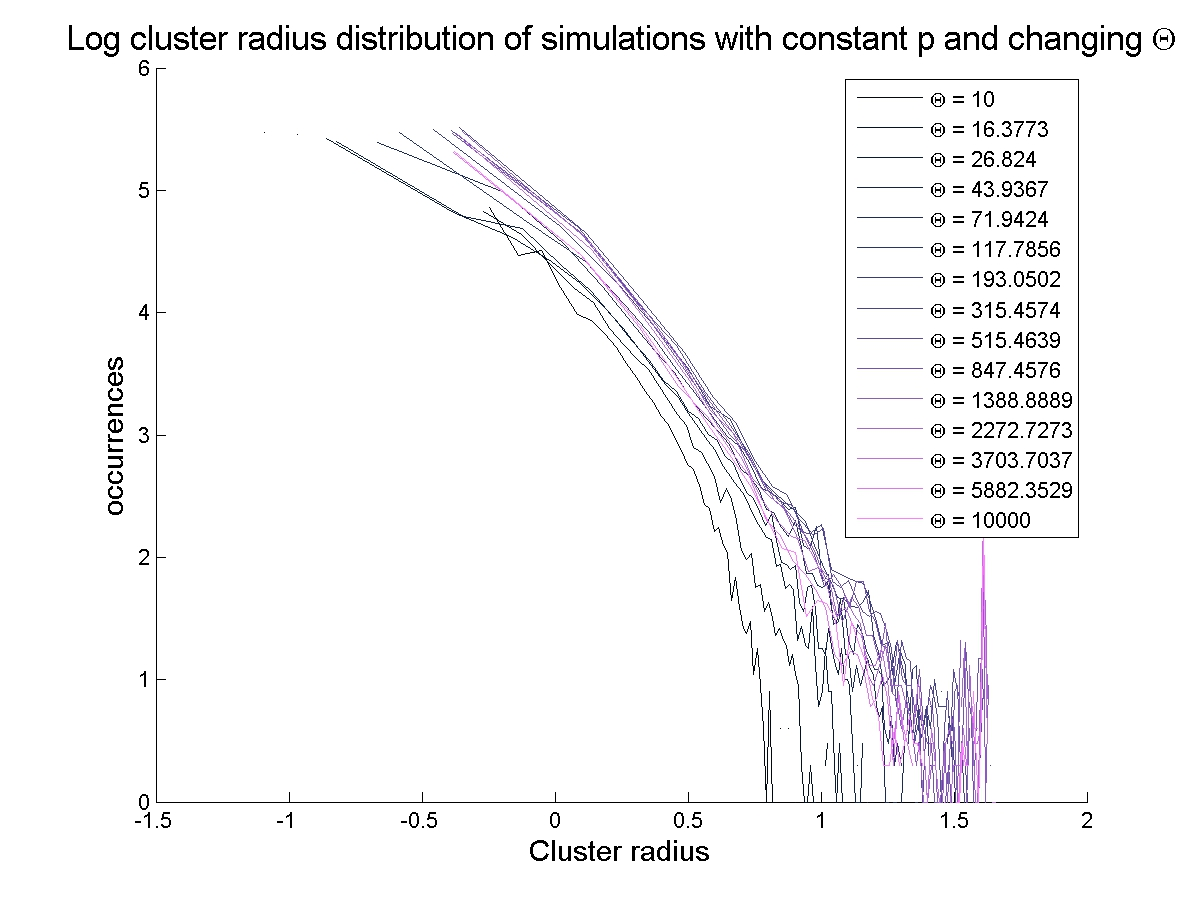
\includegraphics[width=0.9\textwidth,keepaspectratio=true]{Pictures/constpvartheta2.jpg}
\caption{Log cluster radius distributions of simulations with constant p and changing $\Theta$}
\label{varthetaconstp}
\end{figure}
For $\Theta > 70$ we start to see a very consistent slope. Having a lower value, the curves do not anymore fit the pattern and do not exhibit a straight slope. It is important to remember that we only focus on the shape and slope of the curve, not on the location.

\subsubsection{Effect of the grid size}
The third parameter having an impact on the simulation results was the grid size. Since we were applying periodic boundary conditions, it was not clear from the beginning as to what extent this parameter would be important. We run several simulations with all parameters except the grid size fixed. The results are shown in Fig.\ref{vargridsize}.
\begin{figure}[H]
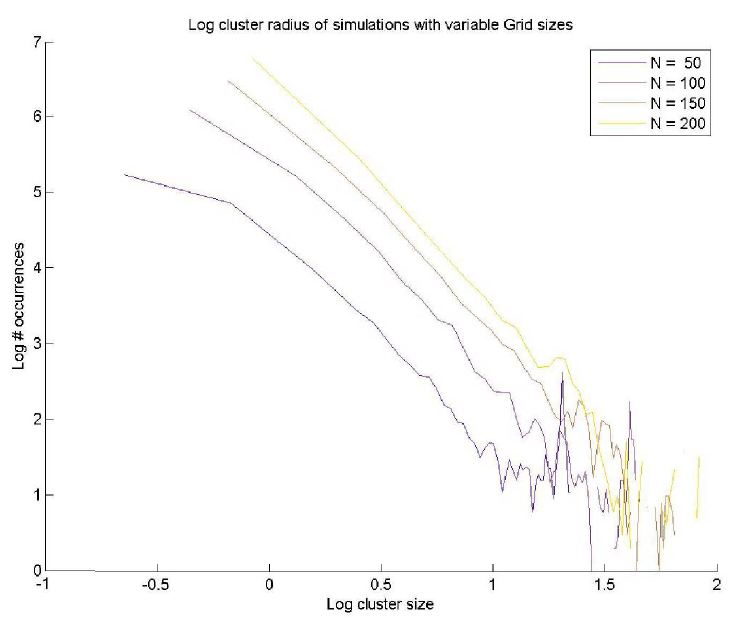
\includegraphics[width=0.9\textwidth,keepaspectratio=true]{Pictures/vargridsize.jpg}
\caption{Log cluster radius distributions with variable grid sizes}
\label{vargridsize}
\end{figure}
Since all the different simulations yield the same slope, we conclude that the grid size only has a marginal impact on the qualitative simulation results.

\subsubsection{Effect of the Initial conditions}
One of the main properties of an SOC state is, that it is an attractor of the system dynamics, much like a minimum potential location. It is stable with respect to small disturbances. If that would not be the case, then the system would not evolve to that state in the first place. Now to check if our state can in fact be an SOC state, it needs to evolve to a certain point independant of the initial conditions. A property of the system, in the Limit $T_{burn} \rightarrow 0$, is, that it is in fact memoryless. Beside the current grid configuration, no other information is used to compute the next iteration. This basically means that if we initialize the system in any starting configuration and end up with an SOC state, we can look at all past grid configurations as initial conditions for (smaller) simulations that have lead to an SOC state. In the course of our simulations, with the right choice of parameters, we thus have possibly created a significant fraction of all possible initial conditions (for a given grid), which have always lead to an SOC state. We therefore conclude that the simulation is \emph{not} dependant on the initial conditions. 

\subsection{Research questions}

To our understanding, the forest fire model exhibits SOC behavior independantly of all parameters except the $p/f$-ratio. Finding an appropriate value is often not too difficult. We have employed simulations with very high values $p/f>N^{2}$, leading the simulation to mostly filling the whole grid before a fire occurs. This does not result in an SOC behavior and is related to finite grid size effects. We have also tried to simulate with $p/f \rightarrow 1$ which has also not lead to satisfying results. We have found that choosing a value of around $p/f \approx N$ will let the system exhibit SOC behavior. A quantitative analysis of theis statement would be very time consuming because the critical threshholds of $p/f$ are most probably dependant on the grid size and therefore have to be tested on a wide range of grid sizes.



\section{Open Questions and Future Scope}
There are certain other concepts which should be understood if one wants to understand Self Organized Criticality. One of the first things is from the basic ideas on SOC, we understand that the system should have certain power law behaviors. But how does one figure out which are the quantities one should be looking at, to find such power laws. One should try to make use of various  mean field theories to find the critical exponents of these power laws.\\
The limited capability of the original model to distinguish an SOC state from other states is most probably because of limited computational capability. It would be an important question to be able to identify an SOC state from this model.
Certain global aspects of SOC have to be searched by applying different boundary conditions and trying to employ different neighborhoods. \\
It is known[ref] that the SOC in Forest Fire model has an an upper critical dimension of 6 which means that for dimensions above 6, the critical exponents calculated from the mean field approaches become exact. In the field of physics, there is also a concept of lower critical dimension which implies that below this critical dimension, there is no phase change. It would be interesting to figure out whether there is any such thing in forest fire model as well.
 







\section{Summary and Outlook}
We were able to reproduce many of the results found in the literature. Looking at the plots, we see a very consistent picture. We have found very prominent power laws regarding the cluster radii and the cluster sizes.\\ 
Yet, after all these simulations, we are still not totally sure if we understood the concept correctly. Though we were able to reproduce the results, we have some doubts about the simulations. We were not able to completely distinguish different phases in the system or differ between equilibria and SOC states. \\
Programming in Matlab is a very fast approach to this sort of problem. It is incredibly convenient and offers a lot of useful built-in functions. But it obviously has its limits. The most prominent was the simulation time. We think that the simulation could have been implemented more efficiently using other programming environments like C++, but since Matlab was the topic of the course, we worked with that. \\
The course helped very much to make the program more efficient. We have learned a lot about how to implement efficient code, structuring data and organizing results in an efficient manner. \\

For lack of time, we were not able to test everything we wanted. What we feel is the most important thing that we missed, is the critical threshold at which a system turns into an SOC state. We were able to compute the critical $f/p$-ratio, but only for one given set of parameters. Since a single Simulation could take as long as half a day if the results had to be good, it was impossible for us to find the dependencies of the critical threshold with other parameters such as the grid size or the fire burning time. We faced similar problems in the implementation of the original model. The original model which is more dynamic and intuitive effectively helped us only in understanding the different states only qualitatively. Because of long computation time, we are unable to distinguish different phases using the original model.\\

The topic of self-organized criticality is an interesting and challenging one. It can explain phenomena which are not understood intuitively and is appliable to a wide variety of problems. 


\bibliographystyle{unsrt}
\bibliography{ref1}  % list here all the bibliographies that

\begin{appendix}
\section{Forest Fire Model- Traditional Implementation}
The following function is used to implement the basic Forest Fire model
\lstinputlisting{Program/Nishant/basic_fire_model_smaller2.m}

The following function gives the distribution of frequency of clusters and the radius of clusters as a function of the size of clusters.
\lstinputlisting{Program/Nishant/cluster_disrtibution2.m}

The following function is used by the $cluster\_distribution2.m$ and $cluster\_distribution2\_iter.m$ function
\lstinputlisting{Program/Nishant/correct_radius_shift_getter.m}

The following function is used by the $cluster\_distribution2.m$ function
\lstinputlisting{Program/Nishant/radius_size_distribution.m}

The following function is used by the $basic\_fire\_model\_smaller2.m$, $cluster\_distribution2.m$, $basic\_fire\_model\_smaller2\_iter.m$ and $cluster\_distribution2\_iter.m$ function
\lstinputlisting{Program/Nishant/neighbour.m}

The following function is used by the $cluster\_distribution2.m$, $basic\_fire\_model\_smaller2\_iter.m$ and $cluster\_distribution2\_iter.m$ function
\lstinputlisting{Program/Nishant/converter.m}

The following function is used by the $cluster\_distribution2.m$, $basic\_fire\_model\_smaller2\_iter.m$ and $cluster\_distribution2\_iter.m$ function
\lstinputlisting{Program/Nishant/changer.m}

The following function is used by the $cluster\_distribution2.m$, $basic\_fire\_model\_smaller2\_iter.m$ and $cluster\_distribution2\_iter.m$ function
\lstinputlisting{Program/Nishant/enforcer.m}

The following function is used to calculate the various distributions by summing the distributions of all the steps (this is required for SOC).
\lstinputlisting{Program/Nishant/basic_fire_model_smaller2_iter.m}

The following function is used by the $cluster\_distribution2\_iter.m$ function
\lstinputlisting{Program/Nishant/cluster_disrtibution2_iter.m}

The following function is used by the $cluster\_distribution2\_iter.m$ function
\lstinputlisting{Program/Nishant/radius_size_distribution_iter.m}




\section{Instantaneous fire implementation}
\lstinputlisting{Program/Michael/ForFire.m}
\lstinputlisting{Program/Michael/diagnostics.m}
\lstinputlisting{Program/Michael/changeIndex.m}
\lstinputlisting{Program/Michael/clusterburn.m}
\lstinputlisting{Program/Michael/getNcIndex.m}
\lstinputlisting{Program/Michael/lowIndex.m}
\lstinputlisting{Program/Michael/neighbor.m}
\lstinputlisting{Program/Michael/computeradius.m}
\end{appendix}
\end{document}  